%\documentclass[pdftex]{beamer}
%\documentclass[notes=show]{beamer}
%\documentclass[xcolor=dvipsnames]{beamer}
\documentclass[notes=show,beamer,compress]{beamer}

\usepackage{amssymb}
\usepackage{latexsym}
\usepackage{amsfonts}
\usepackage{amsmath}
\usepackage[absolute,overlay]{textpos}
\usepackage[english]{babel}
\usepackage[latin1]{inputenc}
%\usepackage{times}
\usepackage[T1]{fontenc}
\usepackage{tikz}
\usetikzlibrary{arrows,positioning} 
\usepackage{graphicx}
\usepackage{bigstrut}
\usepackage{bbm}
\usepackage{mathrsfs}
\usepackage{epsfig}
\usepackage{array}
%\usepackage{natbib}

\tikzstyle{arrow} = [thick,->,>=stealth]

\mode<presentation> {
	%\usetheme[left,width=1.7cm]{Berkeley}
	%\usetheme{default}
	\usetheme{Boadilla}
	\usecolortheme[RGB={103,102,204}]{structure}
	%\usecolortheme{dove}
	\useoutertheme{infolines}
	\setbeamercovered{transparent}
}

%\renewcommand{\familydefault}{cmss}
%\renewcommand{\mathrm}{\mathsf}
%\renewcommand{\textrm}{\textsf}
%\usefonttheme{serif}
\newcommand{\X}{{\mathbf{X}}}
\newcommand{\x}{{\mathbf{x}}}
\newcommand{\E}{\mathsf{E}}
\newcommand{\V}{\mathsf{Var}}


%%%%%%%%%%%%%%%%%%%%%%%%%%%%%%%%%%%%%%%%%%%%%%%%%%%%%%%%%%%%%%%%%%%%%%%%%%%%%%
%         Neue Kommandos f�r fette Mathebuchstaben innerhalb von Formeln     %
%%%%%%%%%%%%%%%%%%%%%%%%%%%%%%%%%%%%%%%%%%%%%%%%%%%%%%%%%%%%%%%%%%%%%%%%%%%%%%
\newcommand{\bom}{\boldmath}
\newcommand{\ubom}{\unboldmath}
\newcommand{\mb}{\mathbf}

\newcommand{\fmalpha}{\mbox{\bom${\alpha}$}}               %Fettes alpha
\newcommand{\fmbeta}{\mbox{\bom${\beta}$}}                 %Fettes beta
\newcommand{\fmgamma}{\mbox{\bom${\gamma}$}}               %Fettes gamma
\newcommand{\fmdelta}{\mbox{\bom${\delta}$}}               %Fettes delta
\newcommand{\fmepsilon}{\mbox{\bom${\epsilon}$}}           %Fettes epsilon
\newcommand{\fmvarepsilon}{\mbox{\bom${\varepsilon}$}}     %Fettes varepsilon
\newcommand{\fmzeta}{\mbox{\bom${\zeta}$}}                 %Fettes zeta
\newcommand{\fmeta}{\mbox{\bom${\eta}$}}                   %Fettes eta
\newcommand{\fmta}{\mbox{\bom${\theta}$}}                  %Fettes theta (ta)
\newcommand{\fmvarta}{\mbox{\bom${\vartheta}$}}         	 %Fettes vartheta (ta)
\newcommand{\fmiota}{\mbox{\bom${\iota}$}}                 %Fettes iota
\newcommand{\fmkappa}{\mbox{\bom${\kappa}$}}               %Fettes kappa
\newcommand{\fmla}{\mbox{\bom${\la}$}}                     %Fettes lambda (la)
\newcommand{\fmmu}{\mbox{\bom${\mu}$}}                     %Fettes mu
\newcommand{\fmnu}{\mbox{\bom${\nu}$}}                     %Fettes nu
\newcommand{\fmxi}{\mbox{\bom${\xi}$}}                     %Fettes xi
\newcommand{\fmo}{\mbox{\bom${\o}$}}                       %Fettes o
\newcommand{\fmpi}{\mbox{\bom${\pi}$}}                     %Fettes pi
\newcommand{\fmvarpi}{\mbox{\bom${\varpi}$}}               %Fettes varpi
\newcommand{\fmrho}{\mbox{\bom${\rho}$}}                   %Fettes rho
\newcommand{\fmvarrho}{\mbox{\bom${\varrho}$}}             %Fettes varrho
\newcommand{\fmsigma}{\mbox{\bom${\sigma}$}}               %Fettes sigma
\newcommand{\fmvarsigma}{\mbox{\bom${\varsigma}$}}         %Fettes varsigma
\newcommand{\fmtau}{\mbox{\bom${\tau}$}}                   %Fettes tau
\newcommand{\fmupsilon}{\mbox{\bom${\upsilon}$}}           %Fettes upsilon
\newcommand{\fmphi}{\mbox{\bom${\phi}$}}                   %Fettes phi
\newcommand{\fmvarphi}{\mbox{\bom${\varphi}$}}             %Fettes varphi
\newcommand{\fmchi}{\mbox{\bom${\chi}$}}                   %Fettes chi
\newcommand{\fmpsi}{\mbox{\bom${\psi}$}}                   %Fettes psi
\newcommand{\fmomega}{\mbox{\bom${\omega}$}}               %Fettes omega
\newcommand{\fmimath}{\mbox{\bom${\imath}$}}               %Fettes imath

\newcommand{\fmv}{\mathnormal{v}}               %v
\newcommand{\fmu}{\mathnormal{u}}               %v
\newcommand{\fme}{\mathnormal{e}}               %v


\setbeamercolor{bibliography entry title}{fg=black}
\setbeamercolor{bibliography entry author}{fg=black}
\setbeamercolor{subsection in toc}{fg=structure}
\setbeamercolor{palette primary}{bg=structure, fg=white}
%\setbeamercolor{palette secondary}{bg=structure, fg=black}
%\setbeamercolor{palette tertiary}{bg=structure, fg=black}
\setbeamercolor{caption name}{fg=black} \setbeamersize{text margin
	left=.8cm} \setbeamersize{text margin right=1cm}
\hypersetup{linkbordercolor={1 0 0}} \setbeamertemplate{navigation
	symbols}{} \setbeamertemplate{headline}[default]

\setbeamertemplate{enumerate items}[default]

\newcounter{transfct}
\newcounter{begbs}
\newcounter{endbs}
\title[Difference in differences]{Econometrics 2}
\subtitle{Difference in differences}
\author[Lychagin \& Mu\c{c}o]{Sergey Lychagin}
\institute[CEU]{CEU}
\date{Winter 2020}


\AtBeginSection[] {
	\begin{frame}<handout:0>
	\frametitle{TOC}
	\tableofcontents[currentsection]
\end{frame}
}

%\AtBeginSubsection[] {
%  \begin{frame}<beamer>
%   \frametitle{Outline}
%    \tableofcontents[currentsection,currentsubsection]
%  \end{frame}
%}

%\beamerdefaultoverlayspecification{<+->}
\begin{document}

\frame{\titlepage}

\begin{frame}{John Snow's study of cholera infection in London}

\begin{itemize}
	\item{Lambeth Company sourced water downstream in 1849, upstream in 1854.}
	\item{Southwark \& Vauxhall sources water downstream in both years.}
\end{itemize} 
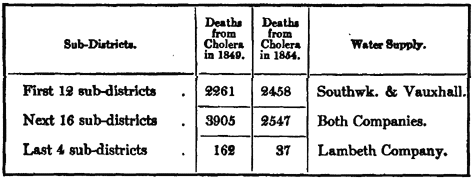
\includegraphics[width=9cm]{graphs/table12.png}

\end{frame}

\begin{frame}{Effect of minimum wage on teenage employment}
	\begin{itemize}
		\item Theory: Lower demand $\Rightarrow$ unemployment
		\item New Jersey: raised minimum wage from $\$4.25$ to $\$5.05$ on April 1, 1992.
	\end{itemize}
	Card and Krueger (1994): ''Minimum Wages and Employment: A Case Study of the Fast Food Industry in New Jersey and Pennsylvania''
\end{frame}

\begin{frame}
\frametitle{Effects of minimum wage change on teenage employment}

\textbf{1. Before-After Design}
\[
Y_{it} = \alpha + \rho D_{it}+ u_{it}
\]

\begin{itemize}
	\item $Y_{it}$ employment of teenage workers in New Jersey fast food restaurants at $t= \text{Feb}, \text{Nov} 1992$, and
	\begin{eqnarray*} D_{it}= \left\{ \begin{array}{cc}
			1 & \text{if}\;\; t=Nov \\
			0 & \text{if}\;\; t=Feb
		\end{array} \right.
	\end{eqnarray*}
	\item  Is $\rho$  causal effect of the minimum wage change? Assumption:
	\begin {itemize}
	\item In absence of minimum wage change $\rho$ would be zero.
	\item No other factors change employment over time.
	\item Change in employment in NJ between February and November only due to change in minimum wage.	
	\end {itemize}
	\end {itemize}
	Very brave assumptions! How about seasonal changes? Business cycle? Other factors?
\end{frame}

\frame{ \frametitle{}
	\begin{center}
		\begin{figure}[t]
			\includegraphics[width=1.1\linewidth]{"graphs/ap_2"}
		\end{figure}
	\end{center}
}


%slide 2

\begin{frame}
\frametitle{Differences in Differences}

\begin{itemize}
\item Panel/repeated CS design where the regressor of interest varies at a more aggregate level
\item Policy changes over time affecting certain population groups, regions, ...
\item OVB: unobserved variables at the state/year/\ldots level: \emph{group fixed effects}.

\end{itemize}
\end{frame}


% slide 3






% slide 4

\begin{frame}
\frametitle{Differences in Differences}

\textbf{2. Before-After Design with Untreated Comparison Group}
\begin{itemize}
\item  Pennsylvania left the minimum wage unchanged in 1992
\item Compare employment change in PA fast food restaurants
\item Potential Outcome:
\begin {itemize}
\item $Y_{1ist}$ restaurant $i$, state $s$, time $t$  with high min. wage
\item  $Y_{0ist}$  with low min wage
\end {itemize}
\end {itemize}

 \begin{eqnarray*}
	          E[ Y_{0ist}| s,t] &=& \gamma_{s} + \lambda_{t} \\
	           E[ Y_{1ist}-Y_{0ist}| s,t] &=& \rho
  \end{eqnarray*}
Let $D_{st}$ be a dummy equal one if minimum wage is high

 \begin{eqnarray*}
  Y_{ist} =\gamma_{s} + \lambda_{t} + \rho D_{st}+ \epsilon_ {ist}
\end{eqnarray*}

\end{frame}




% slide 5

\begin{frame}
\frametitle{Differences in Differences }

 \begin{eqnarray}
 E[Y_{ist}| s=PA, t=Nov]&-& E[Y_{ist}| s=PA, t=Feb]  \nonumber\\
&=& \lambda_{Nov}-\lambda_{Feb} \\
E[Y_{ist}| s=NJ, t=Nov] &-&E[Y_{ist}| s=NJ, t=Feb] \nonumber\\
&=&\lambda_{Nov}-\lambda_{Feb}+ \rho
\end{eqnarray}
Differences in Differences:
\[ (2) - (1) = \rho  \]
 Assumption:
\begin {itemize}
\item In absence of minimum wage change employment in NJ would have developed the same way as in PA
\item No other factors only affect NJ and not PA
\end {itemize}

\end{frame}



%slide 6

\begin{frame}
\frametitle{Regression Diff in Diff}

 \begin{eqnarray*}
Y_{ist}&=& \alpha + \gamma NJ_{s}+ \lambda d_{t}+ \rho ( NJ_{s}\times d_{t})+ \epsilon_{ist}
 \end{eqnarray*}

 \begin{eqnarray*}
NJ_{s} \times d_{t}&=& D_{st} \\
NJ_{s}&=& \left\{ \begin{array}{cc}
                                                1 & \text{if}\;\; s=NJ \\
                                                0 & \text{if}\;\; s=PA
                            \end{array} \right. \\
d_{t}&=& \left\{ \begin{array}{cc}
                                                1 & \text{if}\;\; t=Nov \\
                                                0 & \text{if}\;\; t=Feb
                            \end{array} \right.
 \end{eqnarray*}

Saturated Model
\begin{eqnarray*}
\alpha&=& E[Y_{ist}| s= PA, t= Feb] = \gamma_{PA} + \lambda_{Feb}\\
\gamma&=& E[Y_{ist}| s= NJ, t= Feb]-E[Y_{ist}| s= PA, t= Feb] =\gamma_{NJ} - \gamma_{PA} \\
\lambda&=& E[Y_{ist}| s= PA, t= Nov]-E[Y_{ist}| s= PA, t= Feb] =\lambda_{Nov} - \lambda_{Feb}\\
\rho &=& E[Y_{ist}| s= NJ, t= Nov]-  E[Y_{ist}| s= NJ, t= Feb] \\
&&- \left\{E[Y_{ist}| s= PA, t= Nov]- E[Y_{ist}| s= PA, t= Feb]\right\}
\end{eqnarray*}


\end{frame}







%slide 8


% Why do we need a control? Common trends!

%slide 9
\frame{ \frametitle{}
\begin{center}
\begin{figure}[t]
\includegraphics[width=1.0\linewidth]{"graphs/ap_1"}
\end{figure}
\end{center}
 }



% slide 7

\begin{frame}
\frametitle{Remarks}

 \begin{eqnarray*}
Y_{ist}&=& \alpha + \gamma NJ_{s}+ \lambda d_{t}+ \rho ( NJ_{s}\times d_{t})+ \epsilon_{ist}
 \end{eqnarray*}

\begin {itemize}
\item Main Effects: $NJ_{s}$,  $d_{t}$
\item Interaction $NJ_{s} \times d_{t}$
\item Ideally, we want $\gamma$, $\lambda$ small and $\rho$ big (most convincing).
\item Good to add additional states, time periods
\item{We don't need a panel, a repeated cross section would do just fine}
\end {itemize}
\end{frame}


\begin{frame}{More data from the pre-treatment period?}

Time $t=-\underline{T},\dots,0,1$. Treatment: between $t=0$ and $t=1$. Check if the trends are indeed parallel:
\begin{align*}
Y_{ist} = \sum_{\tau=-\underline{T}}^1\lambda_\tau{}d_{\tau t} + \sum_{\tau=-\underline{T}}^0\gamma_\tau(d_{\tau t}\times{}NJ_s) + \rho (d_{1 t}\times{}NJ_s) + \varepsilon_{ist}
\end{align*}
Test $H_0: \gamma_0 = \gamma_{-1} = \dots = \gamma_{-\underline{T}}$.
\end{frame}

\begin{frame}{No visible co-movement -- bad sign}
In Oct 1996, a federal minimum-wage increase affects PA.
\begin{center}
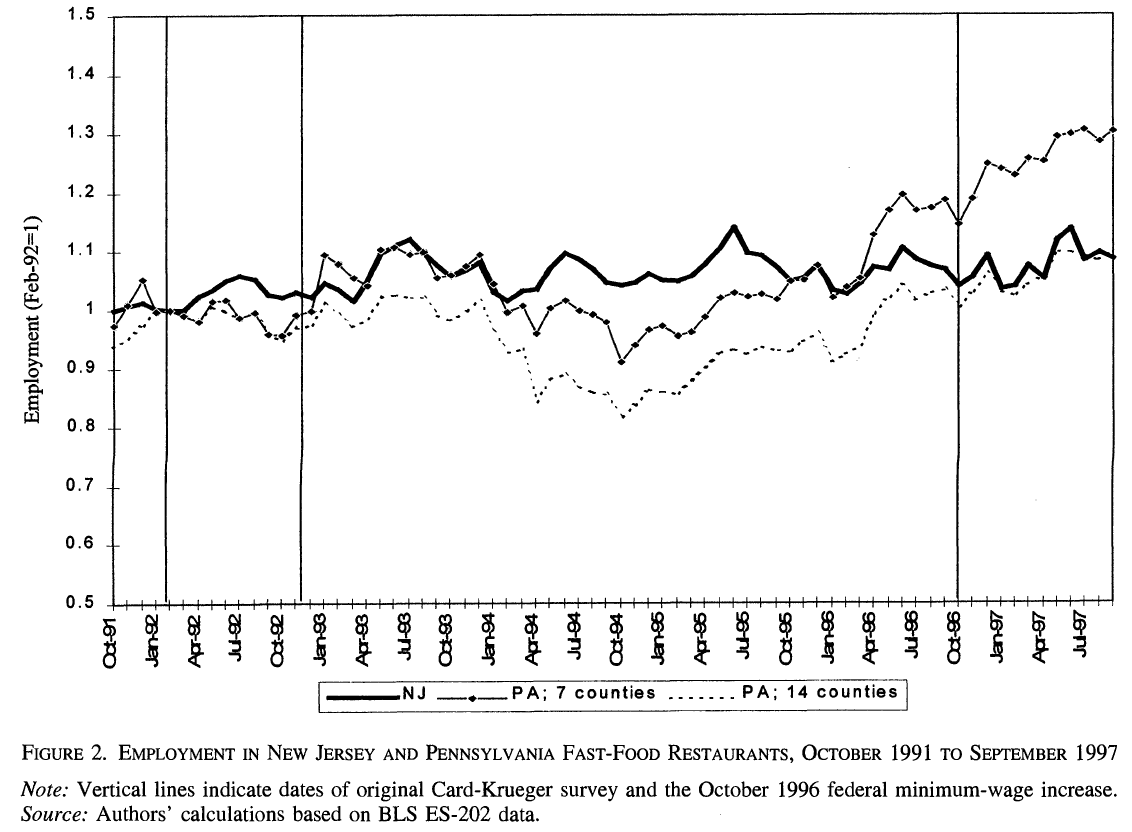
\includegraphics[width=0.75\textwidth]{graphs/card-krueger2000.png}
\end{center}
PA and NJ employment aren't really moving in parallel between '92 and '96.
\end{frame}

\begin{frame}{Ashenfelter's dip -- another bad sign}

Selection based on outcome prior to treatment. Example: effect of a training program on worker earnings. 
\begin{itemize}
	\item{Treatment group: workers who enrolled into training}
	\item{Control: workers who did not.}
	\item{But how do workers self-select into enrollment? Temporary wage decline $\to$ more likely to enroll? Then we have a problem.}
\end{itemize}
Test if $\gamma_0=\gamma_{-1}$.
\end{frame}

\begin{frame}{More data from the post-treatment period?}
Time $t=-\underline{T},\dots, \overline{T}$. Consider delayed effects, set up a fully saturated model. In Card \& Krueger's case, we would estimate
\begin{align*}
Y_{ist} &= \sum_{\tau=-\underline{T}}^{\overline{T}}\lambda_\tau{}d_{\tau t} + \gamma_0NJ_s +  \sum_{\tau=-\underline{T}}^{-1}\gamma_\tau d_{\tau t}\times{}NJ_s\\
&+ \sum_{\tau=1}^{\overline{T}}\rho_\tau d_{\tau t}\times{}NJ_s + \varepsilon_{ist}
\end{align*}
Labor market frictions $\to$ effect of treatment is gradual, $|\rho_2|>|\rho_1|$.
\end{frame}

\begin{frame}{Multiple periods: beware of serial correlation!}

Consider an absurd variation of Card \& Krueger:
\begin{itemize}
	\item{We start with 4 observations: 1 month before/after wage increase, for PA and NJ. Too small of a sample!}
	\item{We obtain employment in PA and NJ at an \emph{hourly} frequency. Large sample, hourly variation is small $\to$ very tight estimates!}
	\item{This must feel wrong, though!}
\end{itemize}
Employment in PA now is likely to be approx. the same as one hour ago. Serial correlation $\rightarrow$ need to adjust std. errors.
\begin{itemize}
	\item{Quick fix: cluster at the level of treatment unit. But then we are left with 2 clusters: NJ and PA.}
	\item{Cluster by county? What about spatial correlation?}
\end{itemize}
To learn more, check Bertrand et al. ``How much should we trust diff-in-diff estimates?''
\end{frame}

\begin{frame}{Treatment in waves (staggered treatment)}
	Example: access to broadband internet. Does it affect economic outcomes (jobs, wages, sales)?
	\begin{itemize}
		\item{Every unit $i$ (a city or a village) is treated at some point. $c$ -- treatment cohort: all units in $c$ get internet access at $t=c$.}
		\item{Idea: use untreated cohorts as a control group for treated cohorts.}
		\item{Assume same effect across cohorts, parallel trends; estimate
			\begin{equation*}
				Y_{ict} = \gamma_c + \lambda_t + \sum_{\tau\geq c}\rho_{\tau-c}d_{\tau t} + \varepsilon_{it}
			\end{equation*}
			Control for $\gamma_c$ and $\lambda_t$ using dummies.}
		\item{$\gamma_c$ --- cohort assignment can be based on the level of $Y$}
	\end{itemize}

\end{frame}

\begin{frame}{Continuous treatment}
Example (a term paper $\approx$5 years ago):
\begin{itemize}
	\item{Construction of a radar in P\'ecs. The locals are unhappy about the project (health, safety concerns).}
	\item{Any effect on real estate prices? Mechanism: lower demand for properties close to the site $\to$ prices drop.}
	\item{Treatment = distance to the radar site. $t=0,1$ --- before/after the announcement, $i$ -- sales ad
	\begin{equation*}
		Y_{it} = \alpha + \gamma{}DIST_i + \lambda{}d_{1t} + \rho{d_{1t}\times{}DIST_i} + \varepsilon_{it}
	\end{equation*}}
	\item{Any obvious issues?}
\end{itemize}
\end{frame}

\begin{frame}{Diff-in-diff and controls}
Selection: properties close to the radar site are different from those in the city center. Different market segments $\to$ different price trends.

Control for $X_{it}$ -- house type, area, distance to schools, etc:
\begin{equation*}
Y_{it} = \alpha + \gamma{}DIST_i + \lambda{}d_{1t} + \rho{d_{1t}\times{}DIST_i} + \beta{}X_{it}+ \varepsilon_{it}
\end{equation*}
$\beta{}X_{it}$ isn't causal; it helps soak up differences in trends between treatment/control group.
\end{frame}



\begin{frame}{Triple differences}
Example: Bisztray ``The effect of FDI on local suppliers''
\begin{itemize}
	\item{Treatment: Audi opens a plant in Gy\H{o}r}. Do local suppliers become more productive?
	\item{Treated firms: (a) produce car parts, (b) are located in Gy\H{o}r.}
	\item{Same industry, other locations --- control for industry-specific shocks.}
	\item{Same location, other industries --- shocks specific to Gy\H{o}r.}
	\item{Other locations, other industries --- overall economy trends.}
	\begin{align*}
		TFP_{it} &= \alpha + \gamma{}GYOR_i + \beta{}SUPPLIER_i + \lambda{}POST_t \\
		&+ \phi SUPPLIER_i\times POST_t + \psi GYOR_i\times POST_t\\
		&+ \delta SUPPLIER_i\times GYOR_i\\
		&+ \rho SUPPLIER_i\times GYOR_i\times POST_t + \varepsilon_{it}
	\end{align*}
	\item{Effect of interest: $\rho$}
\end{itemize}

\end{frame}
\end{document}